\documentclass{zc-ust-hw}

\usepackage{lipsum}

\name{SalahDin Ahmed Salh Rezk}
\id{202201079}
\course{Introduction to Electronics (CIE 212)}
\assignment{Lab Report 1}

\begin{document}

\maketitle

\section{Lab Experiment 1: Half Wave Rectifier}

    \begin{figure}[htbp]
      \centering
      \begin{subfigure}{0.5\textwidth}
        \centering
        \begin{circuitikz}[scale=1.5]
          \draw (0,0) to[sV, l=$V_{in}$] (0,2)
          to[diode, l=D] (2,2)
          to[R, l=R] (2,0)
          -- (0,0);
          \draw (2,2) -- (4,2)
          to[short, -o] (4,1.5)
          to[open, v^=$V_{out}$] (4,0.5)
          to[short, o-] (4,0);
          \draw (2,0) -- (4,0);
        \end{circuitikz}
        \caption{}
      \end{subfigure}%
      \begin{subfigure}{0.5\textwidth}
        \centering
        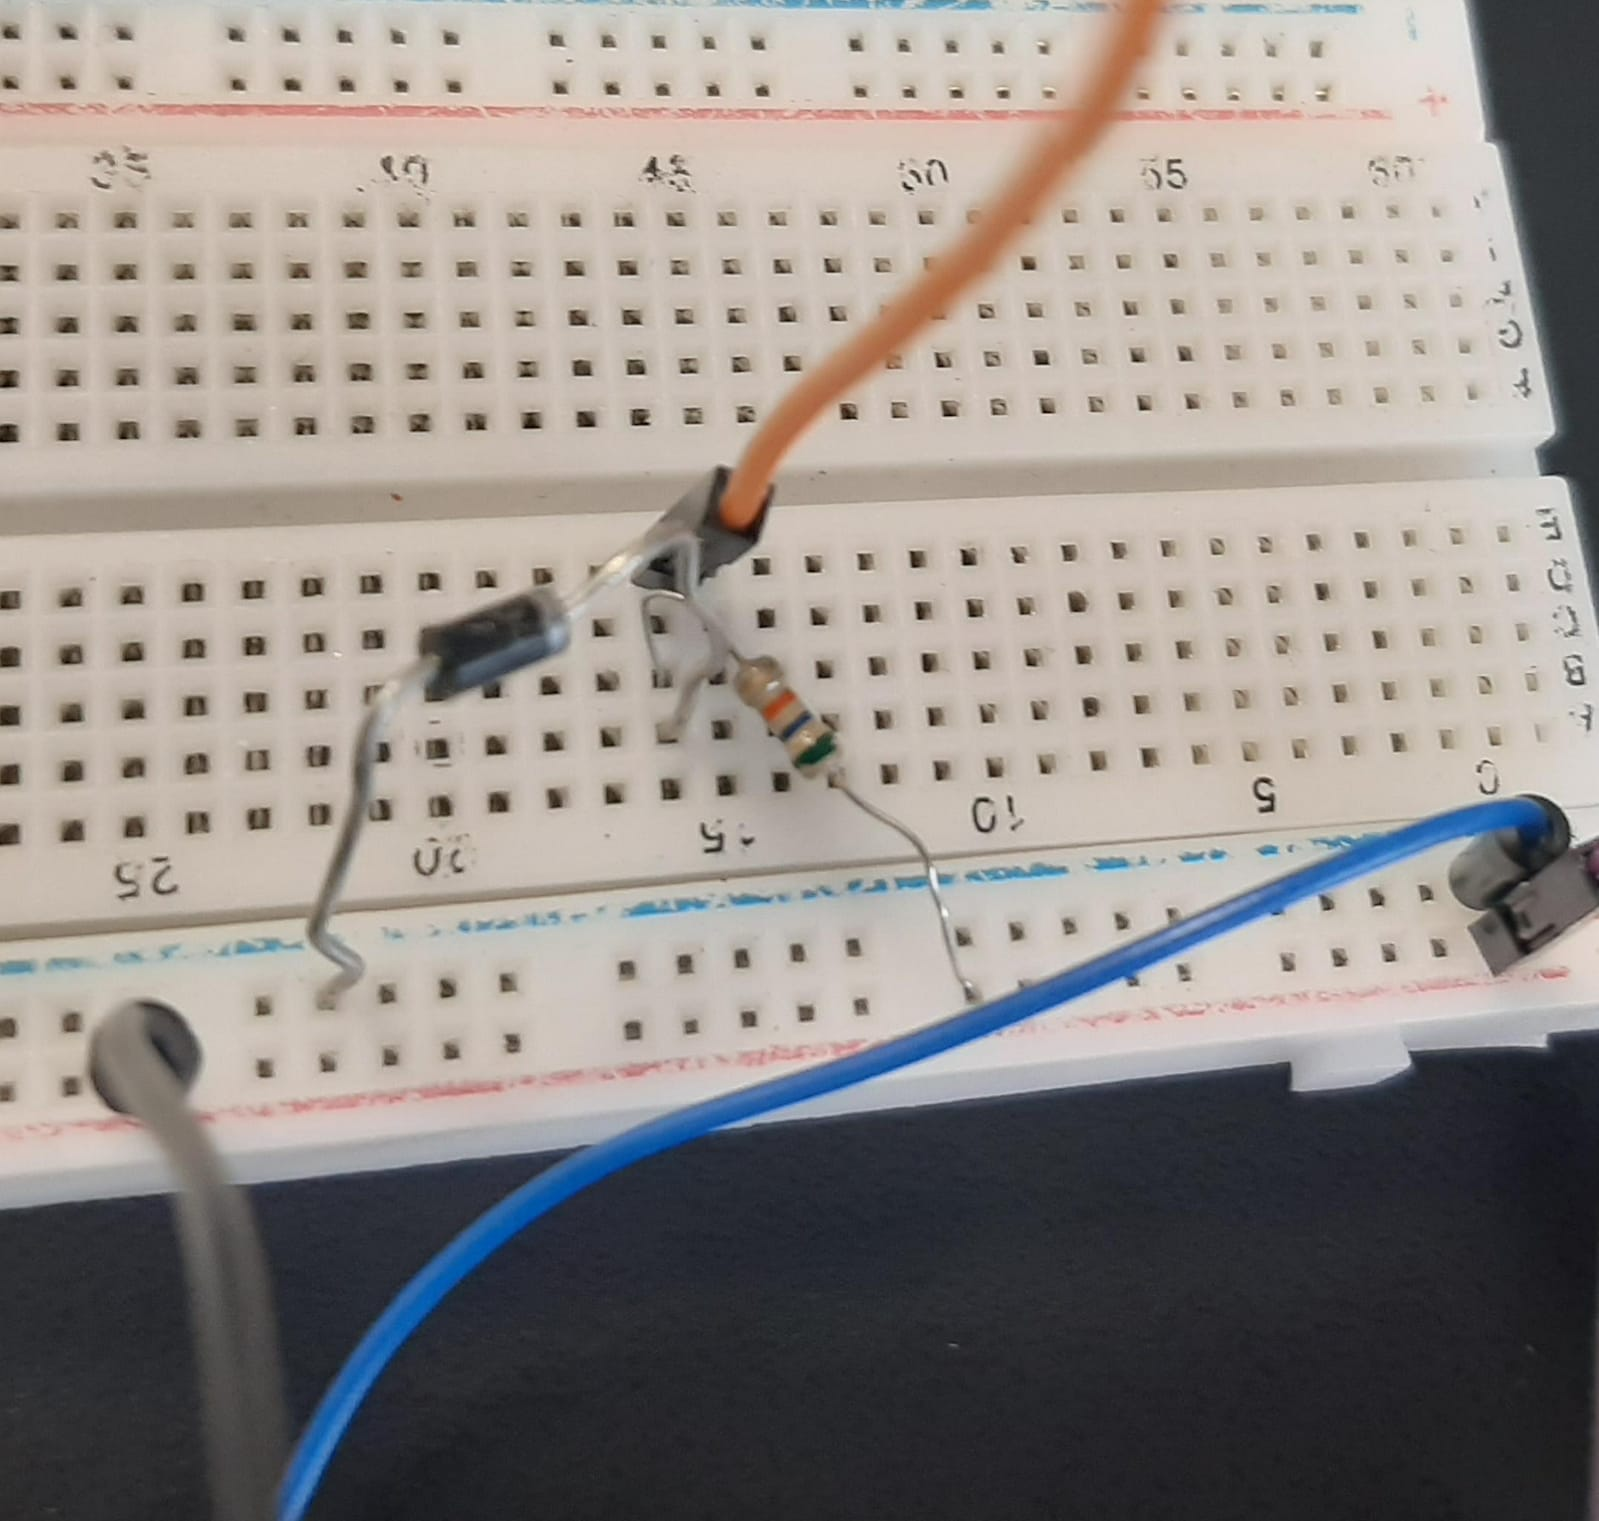
\includegraphics[width=0.5\textwidth]{figures/circuit.jpeg}
        \caption{}
      \end{subfigure}
      \caption{Half Wave Rectifier Circuit}
    \end{figure}

    \begin{figure}[htbp]
      \centering
      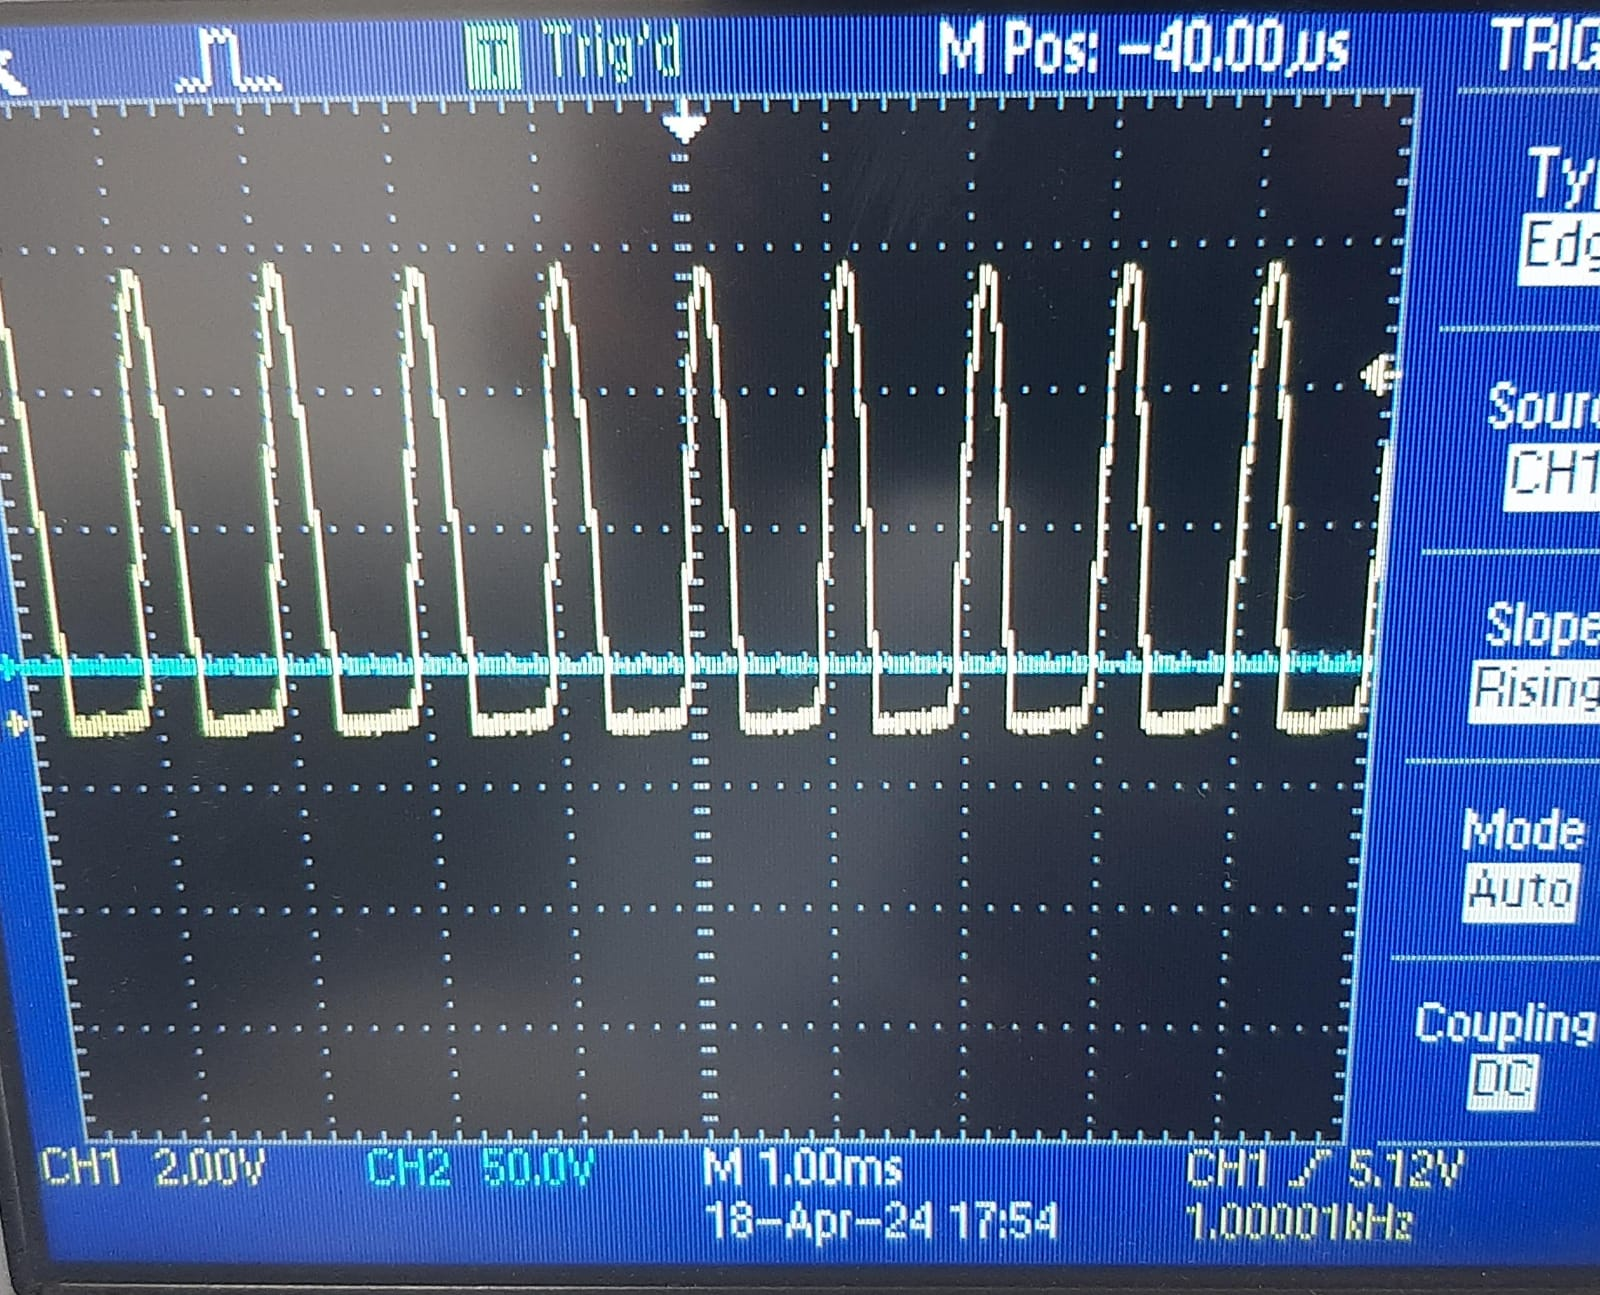
\includegraphics[width=0.5\textwidth]{figures/output.jpeg}
      \caption{Output Voltage Waveform}
    \end{figure}

    \newpage

\section{Lab Experiment 2: Full Wave Rectifier}

We did not perform this experiment.

\section{Lab Assignment}

\begin{enumerate}
  \item \,
    \begin{figure}[H]
      \centering
      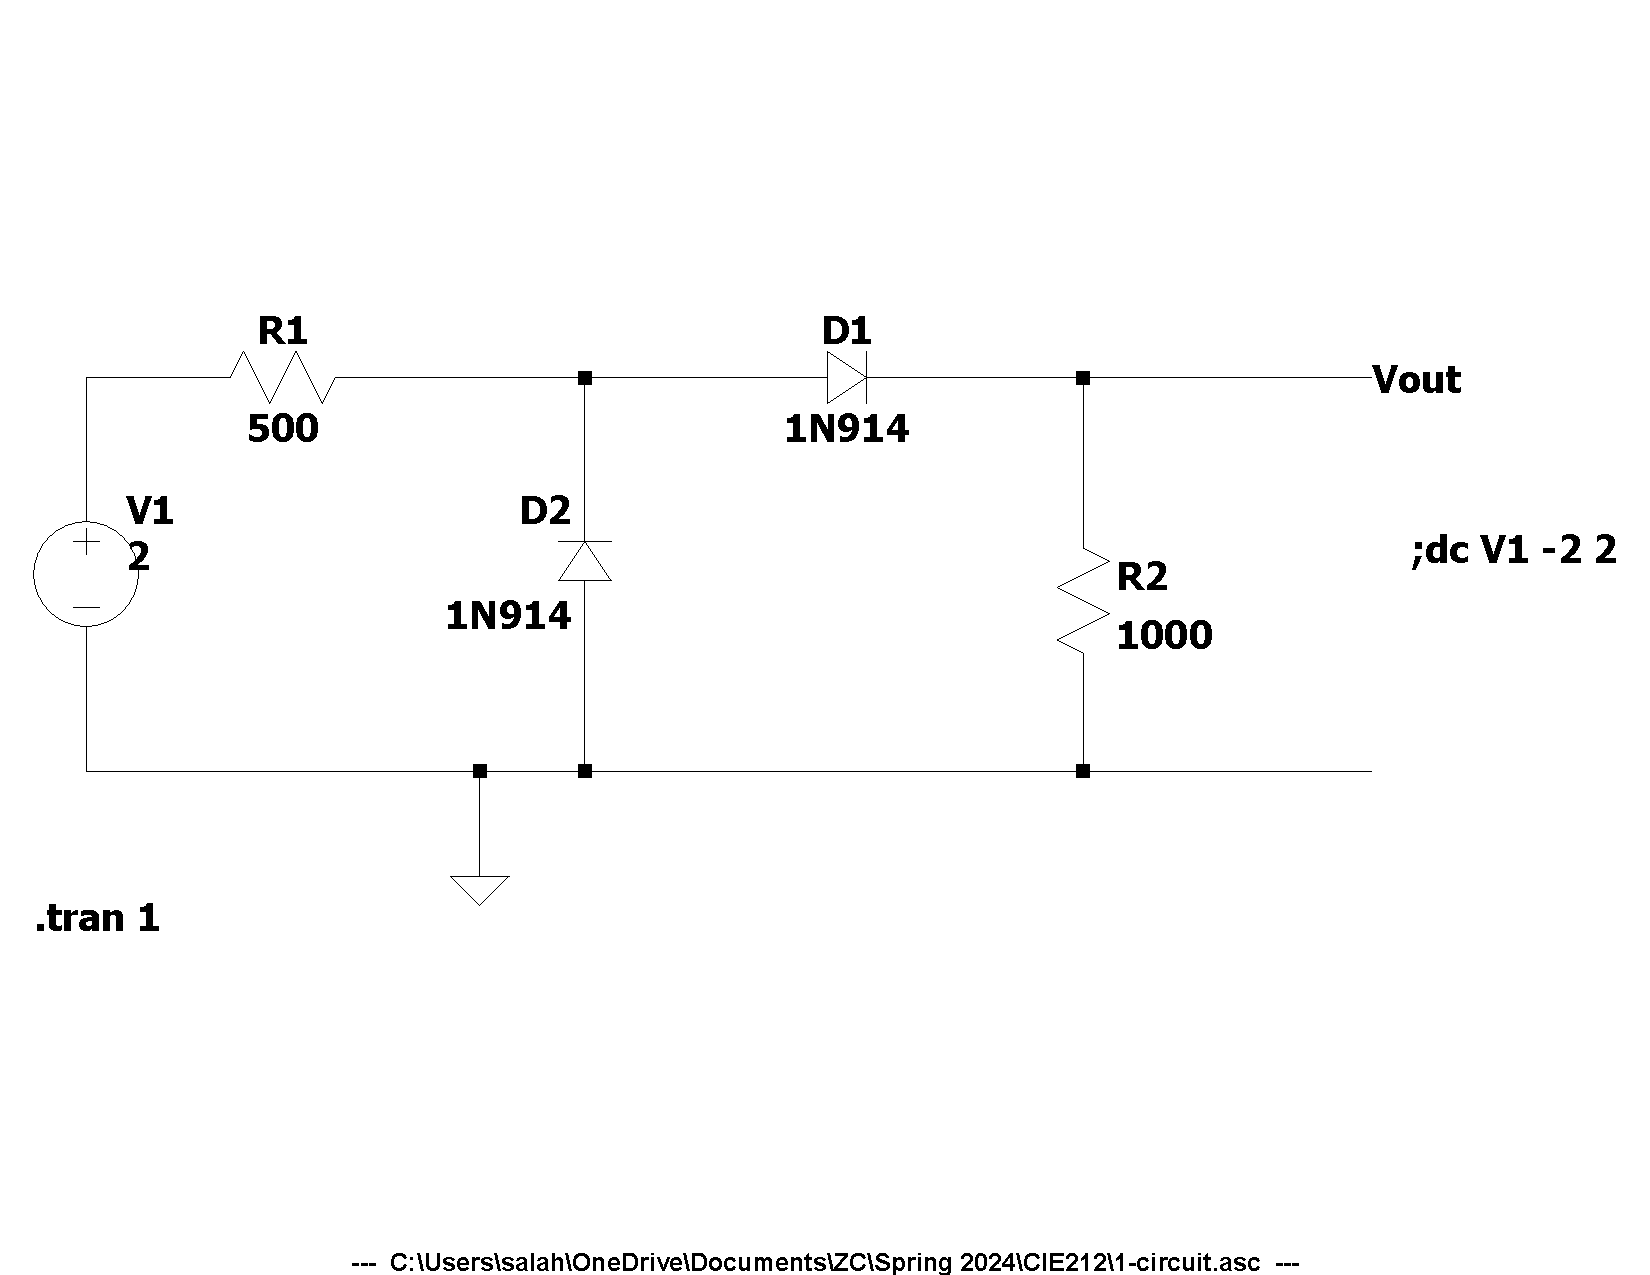
\includegraphics[width=0.95\textwidth]{figures/1-circuit.pdf}
      \caption{Circuit Diagram}
    \end{figure}
    \begin{figure}[H]
      \centering
      \begin{subfigure}{0.45\textwidth}
        \centering
        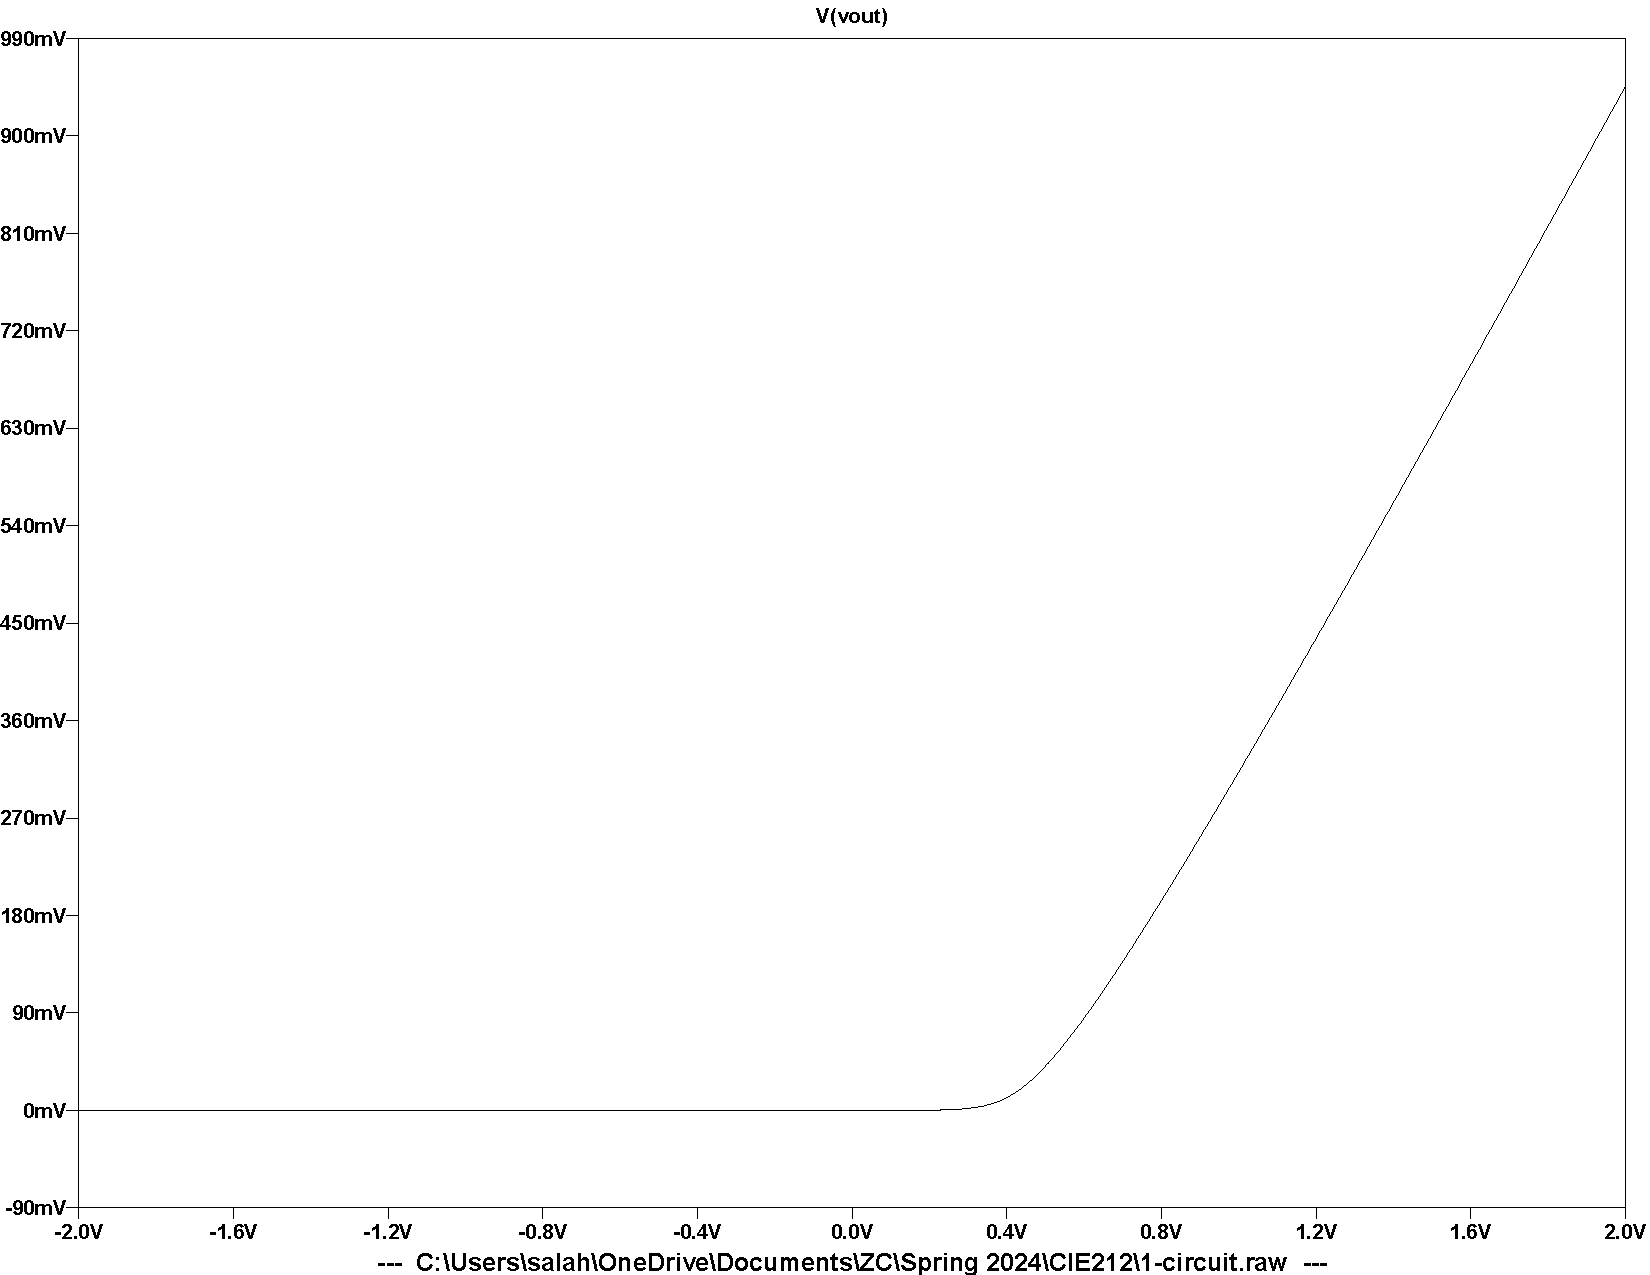
\includegraphics[width=\textwidth]{figures/1-dc-sweep.pdf}
        \caption{DC Sweep}
      \end{subfigure}%
      \begin{subfigure}{0.45\textwidth}
        \centering
        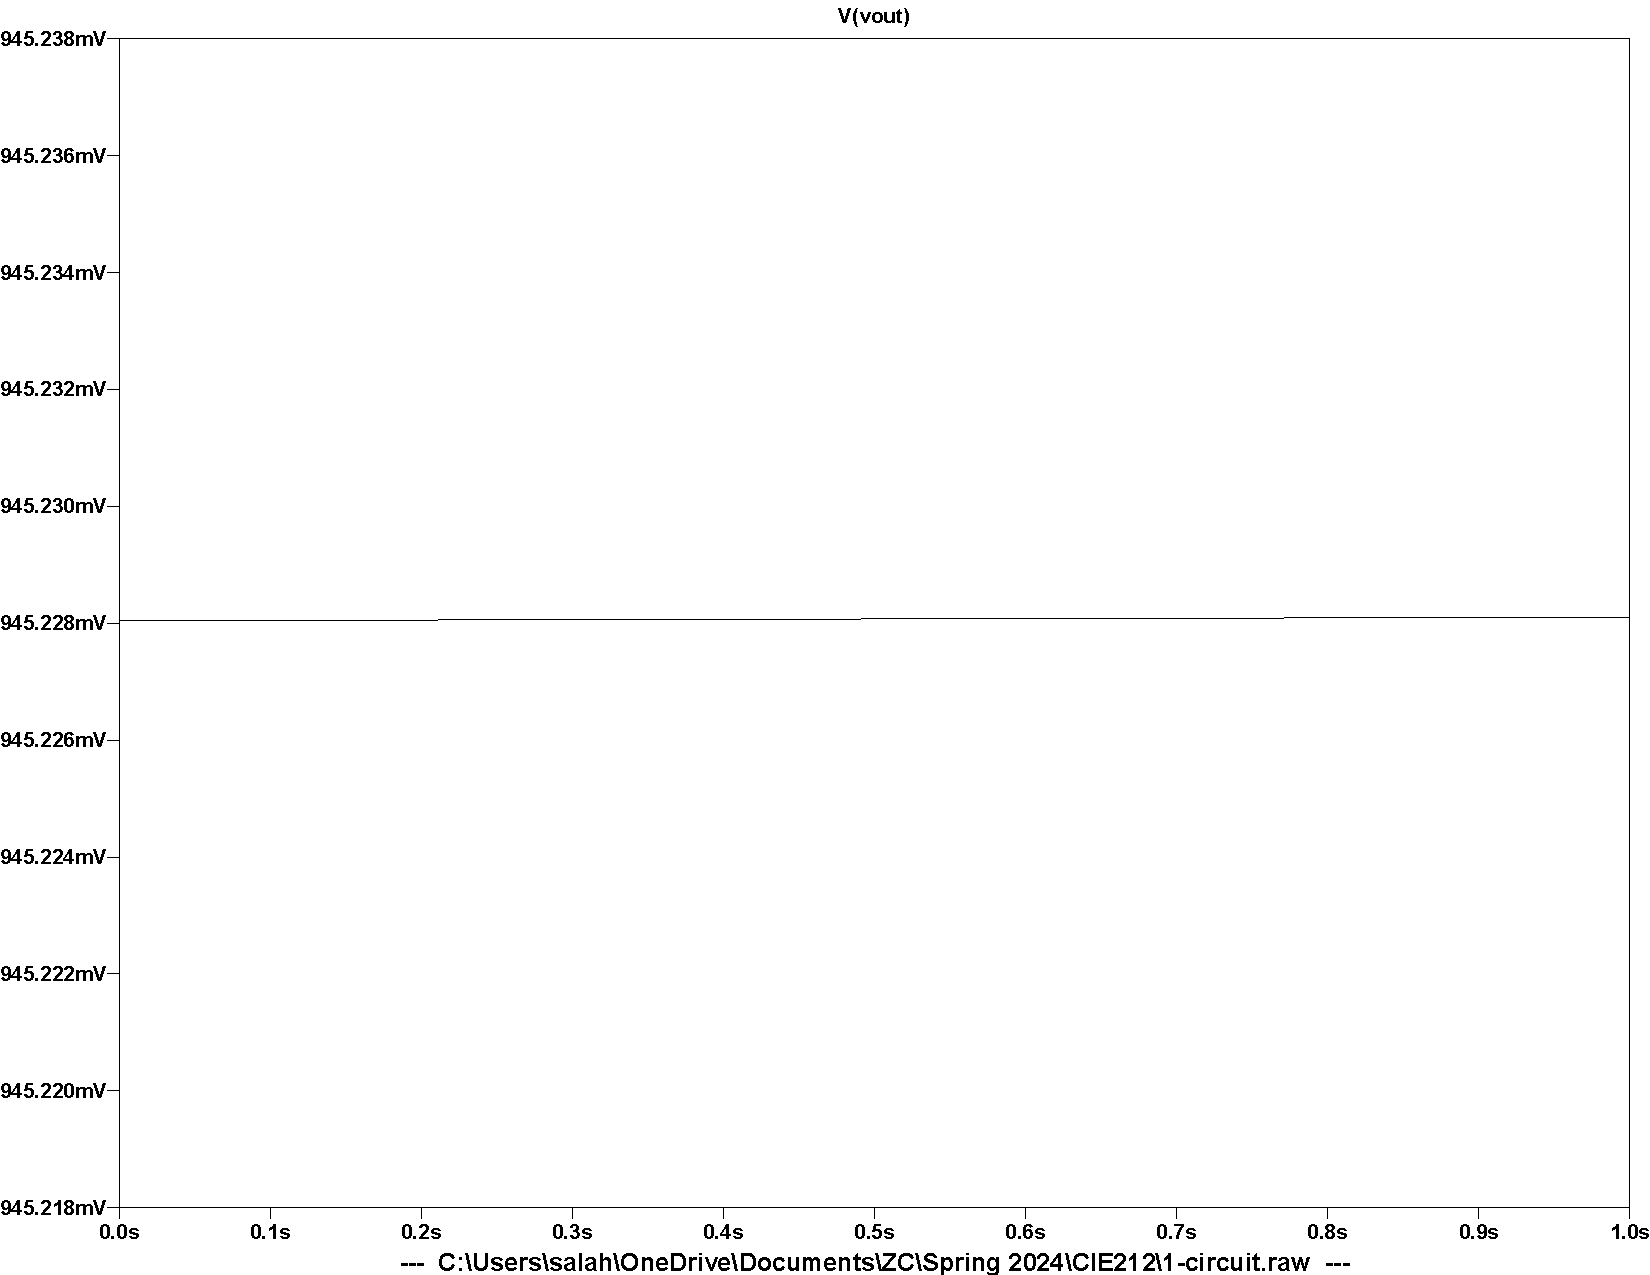
\includegraphics[width=\textwidth]{figures/1-transient.pdf}
        \caption{Transient Analysis}
      \end{subfigure}
      \caption{Simulation Results}
    \end{figure}
    
    \newpage

  \item \,
    \begin{figure}[H]
      \centering
      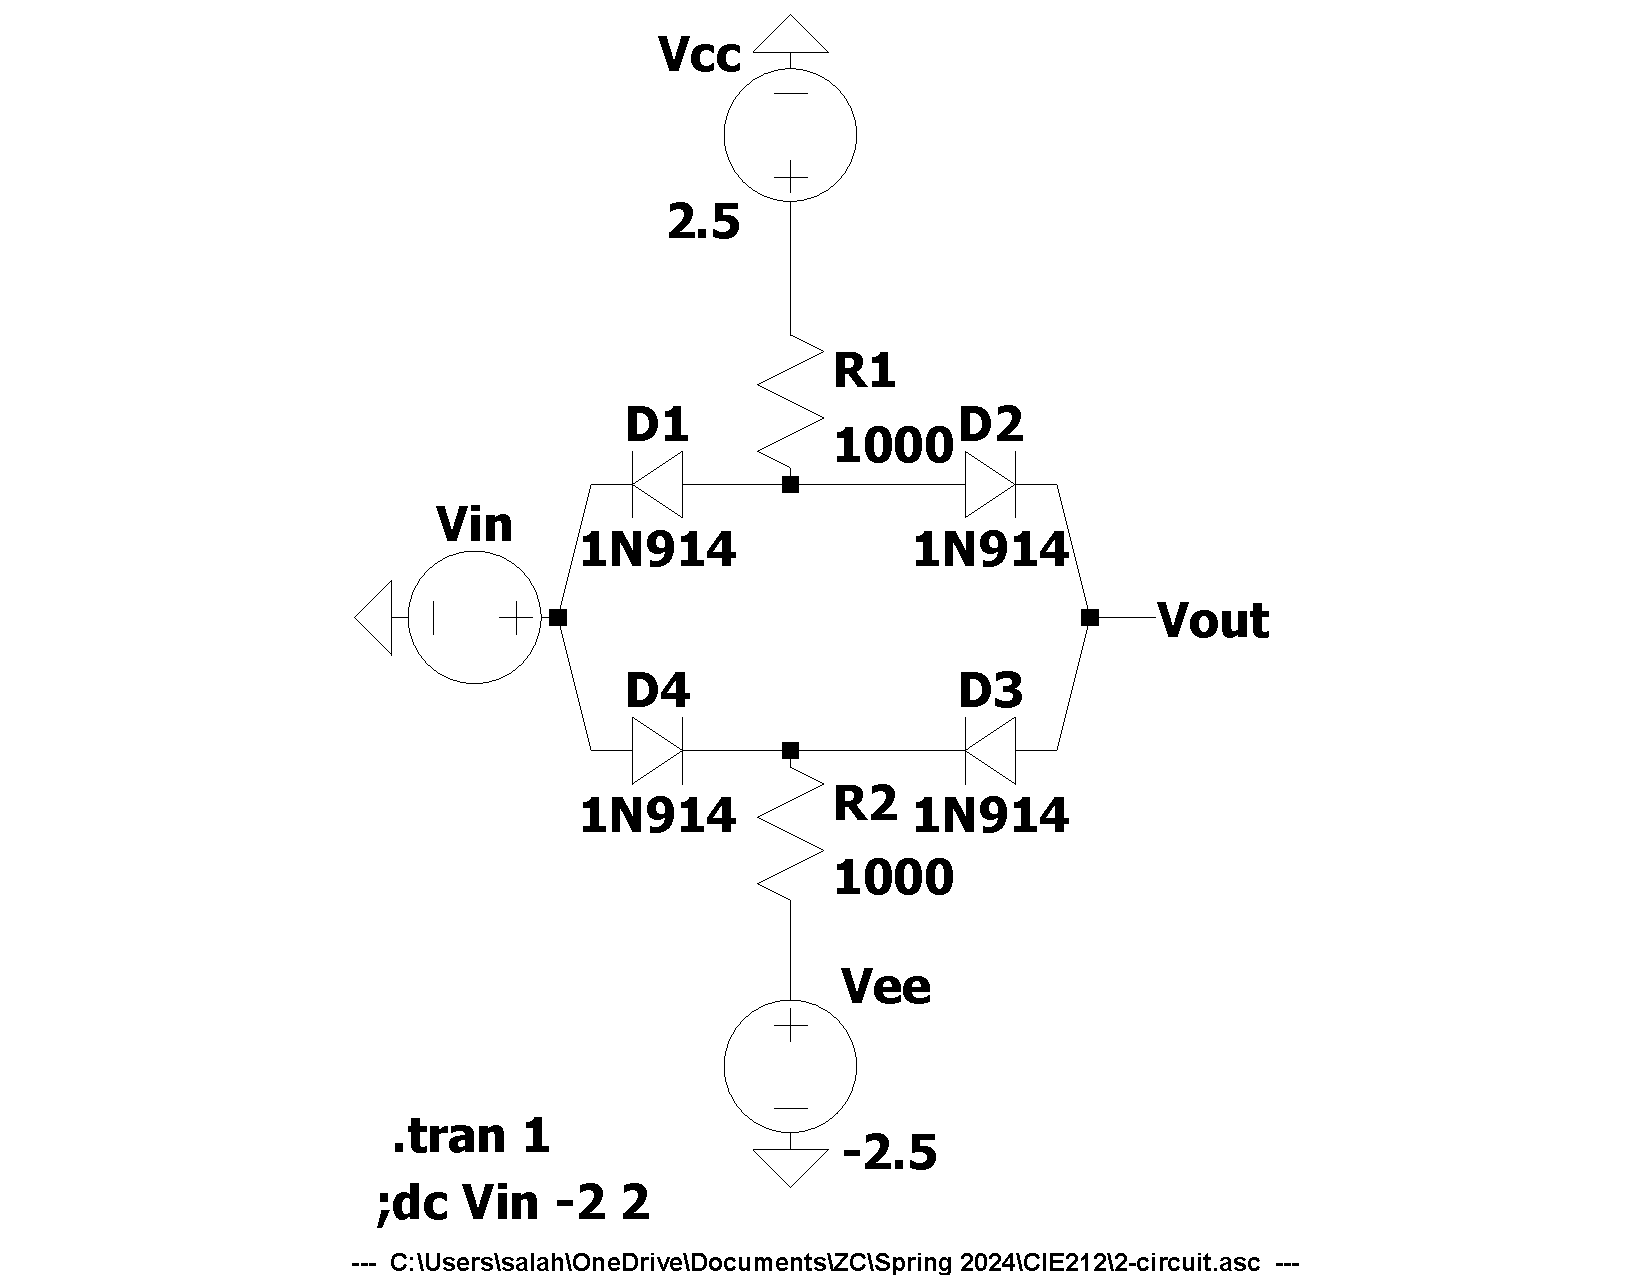
\includegraphics[width=0.95\textwidth]{figures/2-circuit.pdf}
      \caption{Circuit Diagram}
    \end{figure}
    \begin{figure}[H]
      \centering
      \begin{subfigure}{0.45\textwidth}
        \centering
        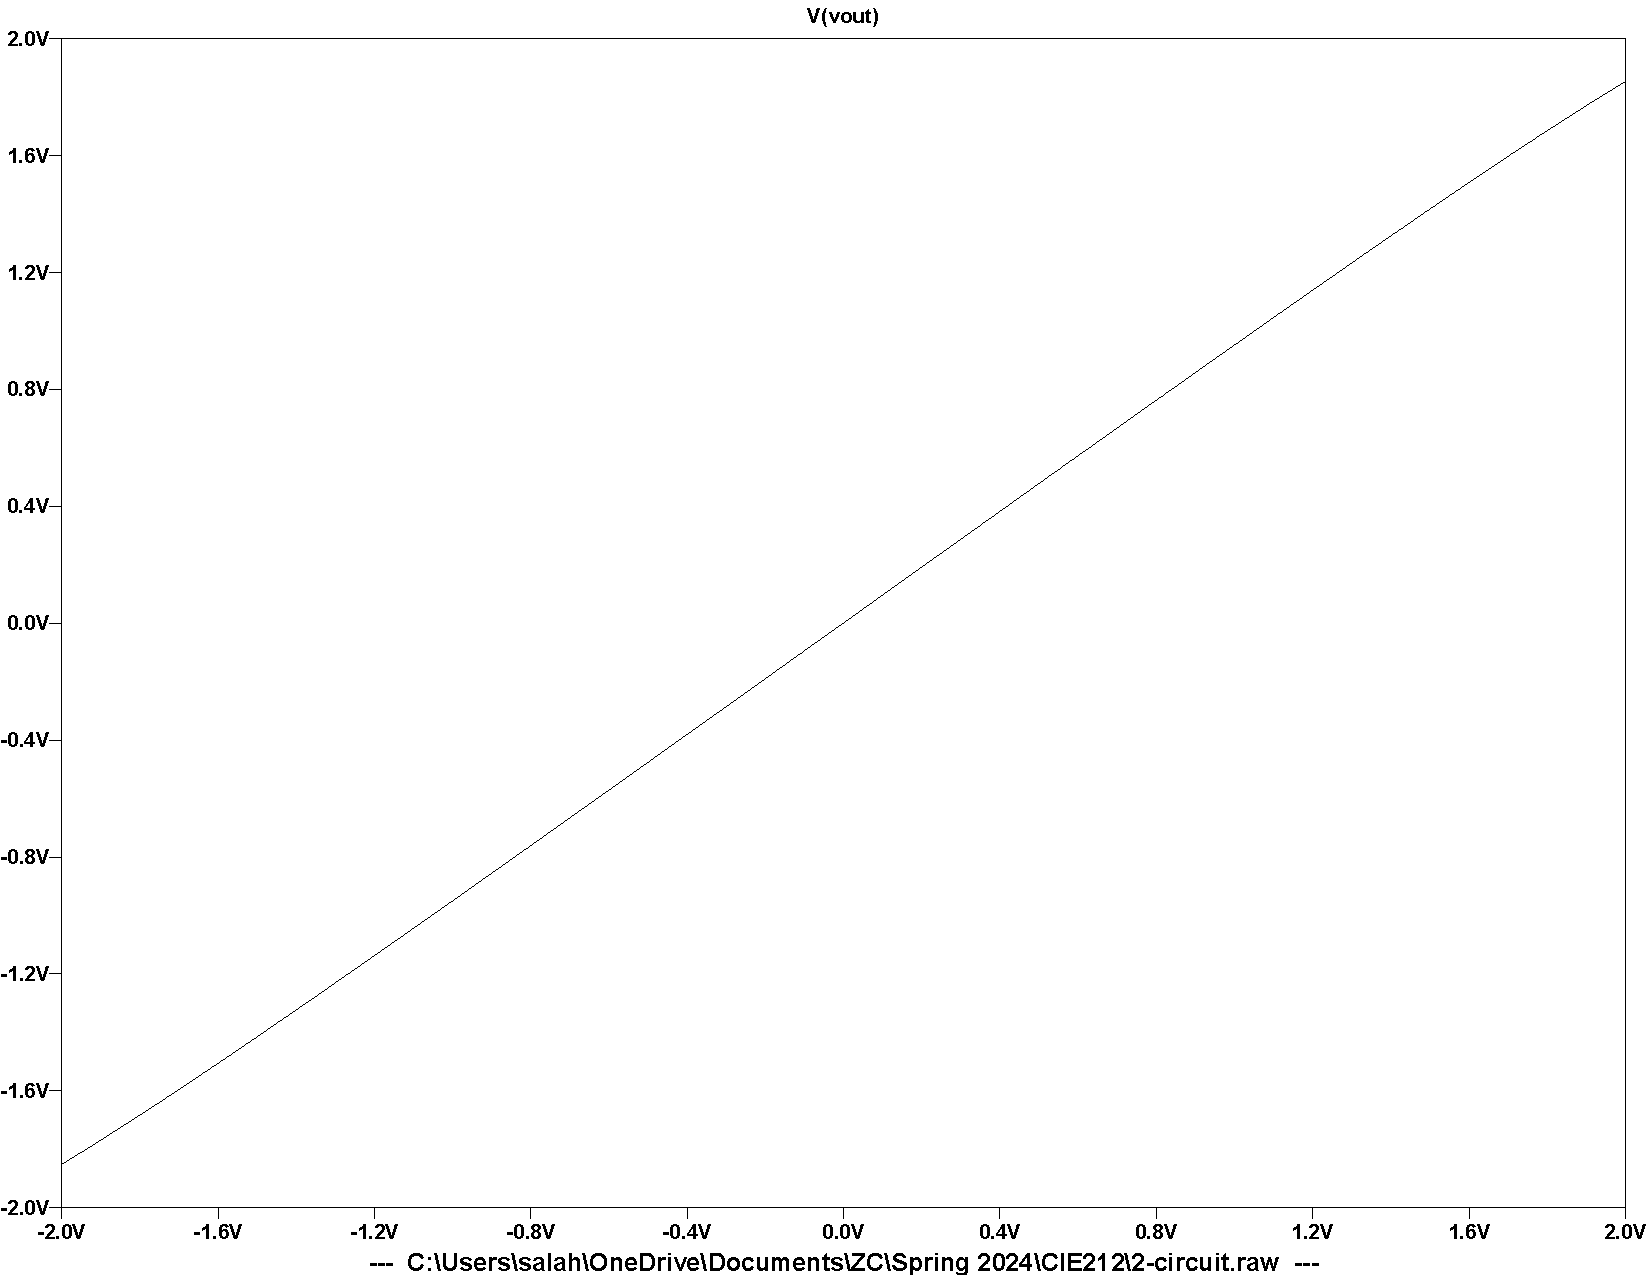
\includegraphics[width=\textwidth]{figures/2-dc-sweep.pdf}
        \caption{DC Sweep}
      \end{subfigure}%
      \vspace{1cm}
      \begin{subfigure}{0.45\textwidth}
        \centering
        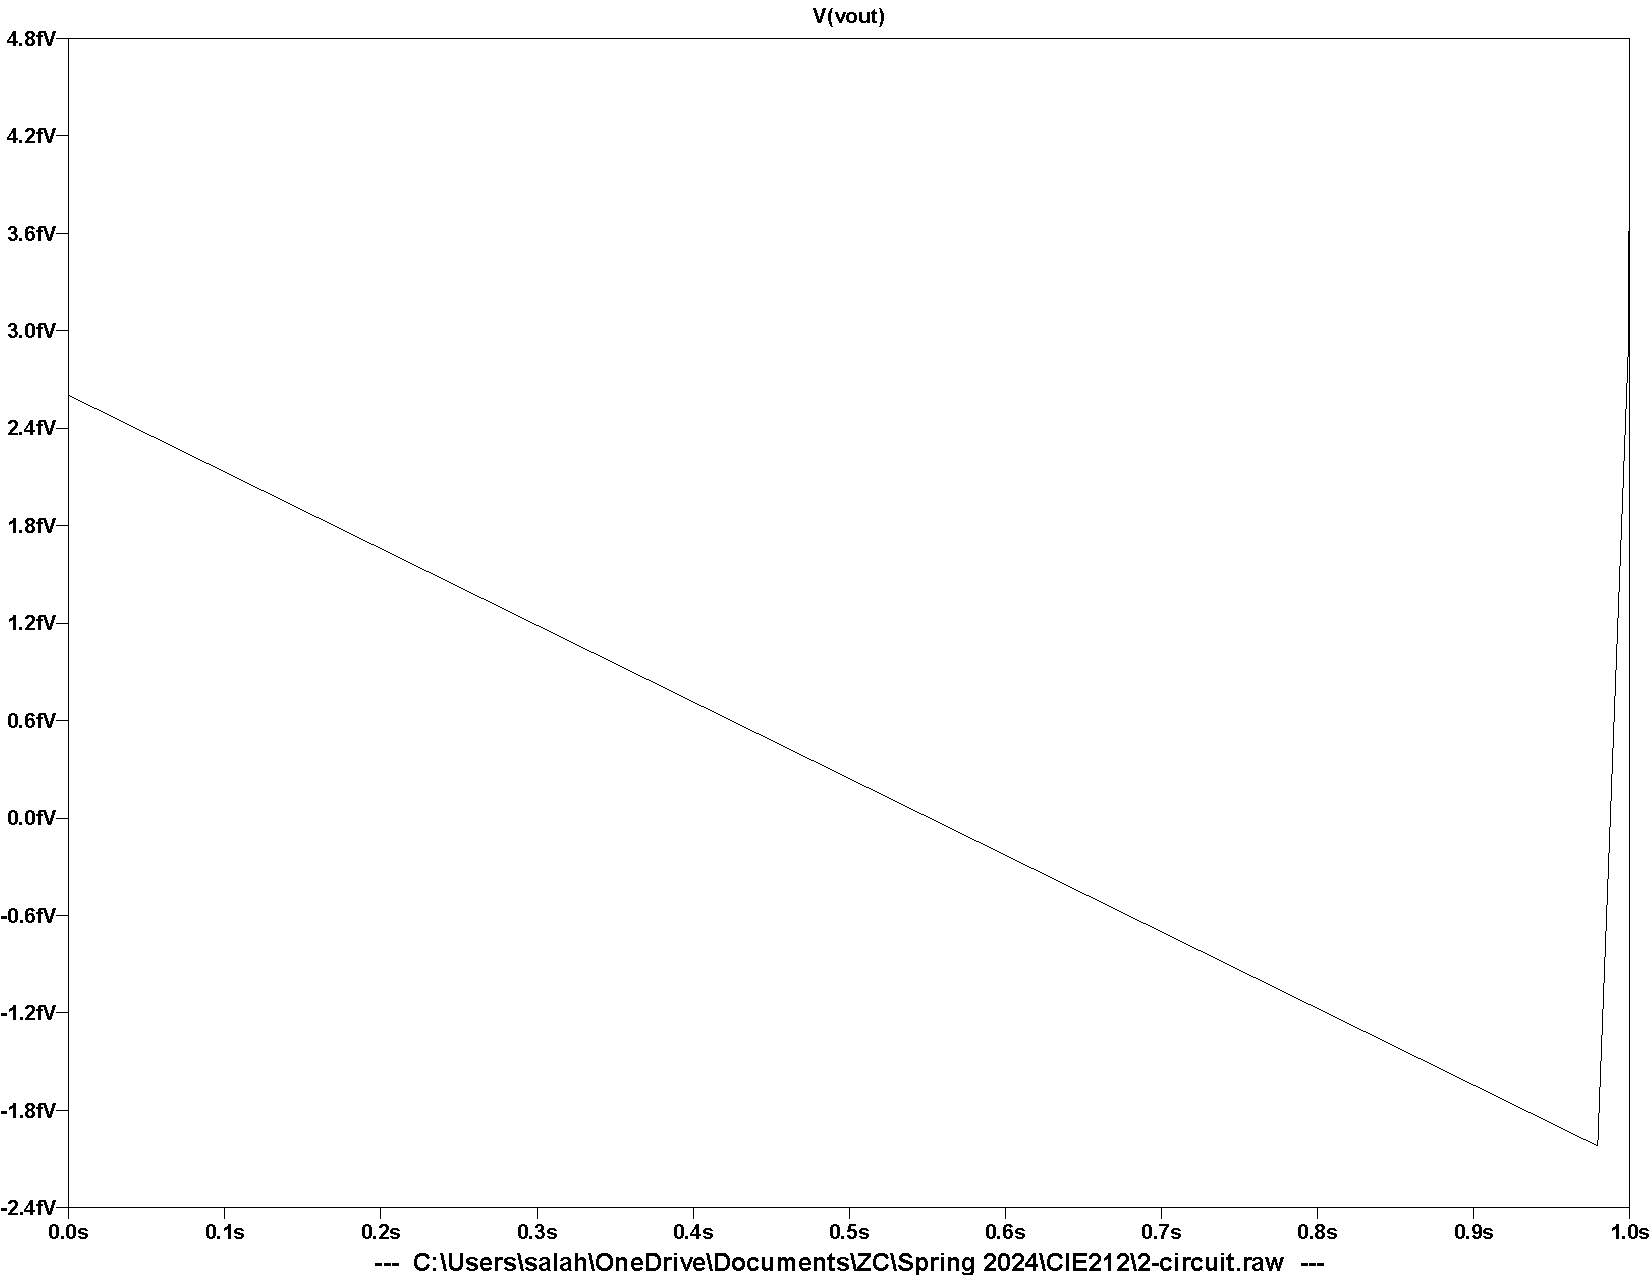
\includegraphics[width=\textwidth]{figures/2-transient.pdf}
        \caption{Transient Analysis}
      \end{subfigure}
      \caption{Simulation Results}
    \end{figure}

    \newpage

  \item \,
    \begin{figure}[H]
      \centering
      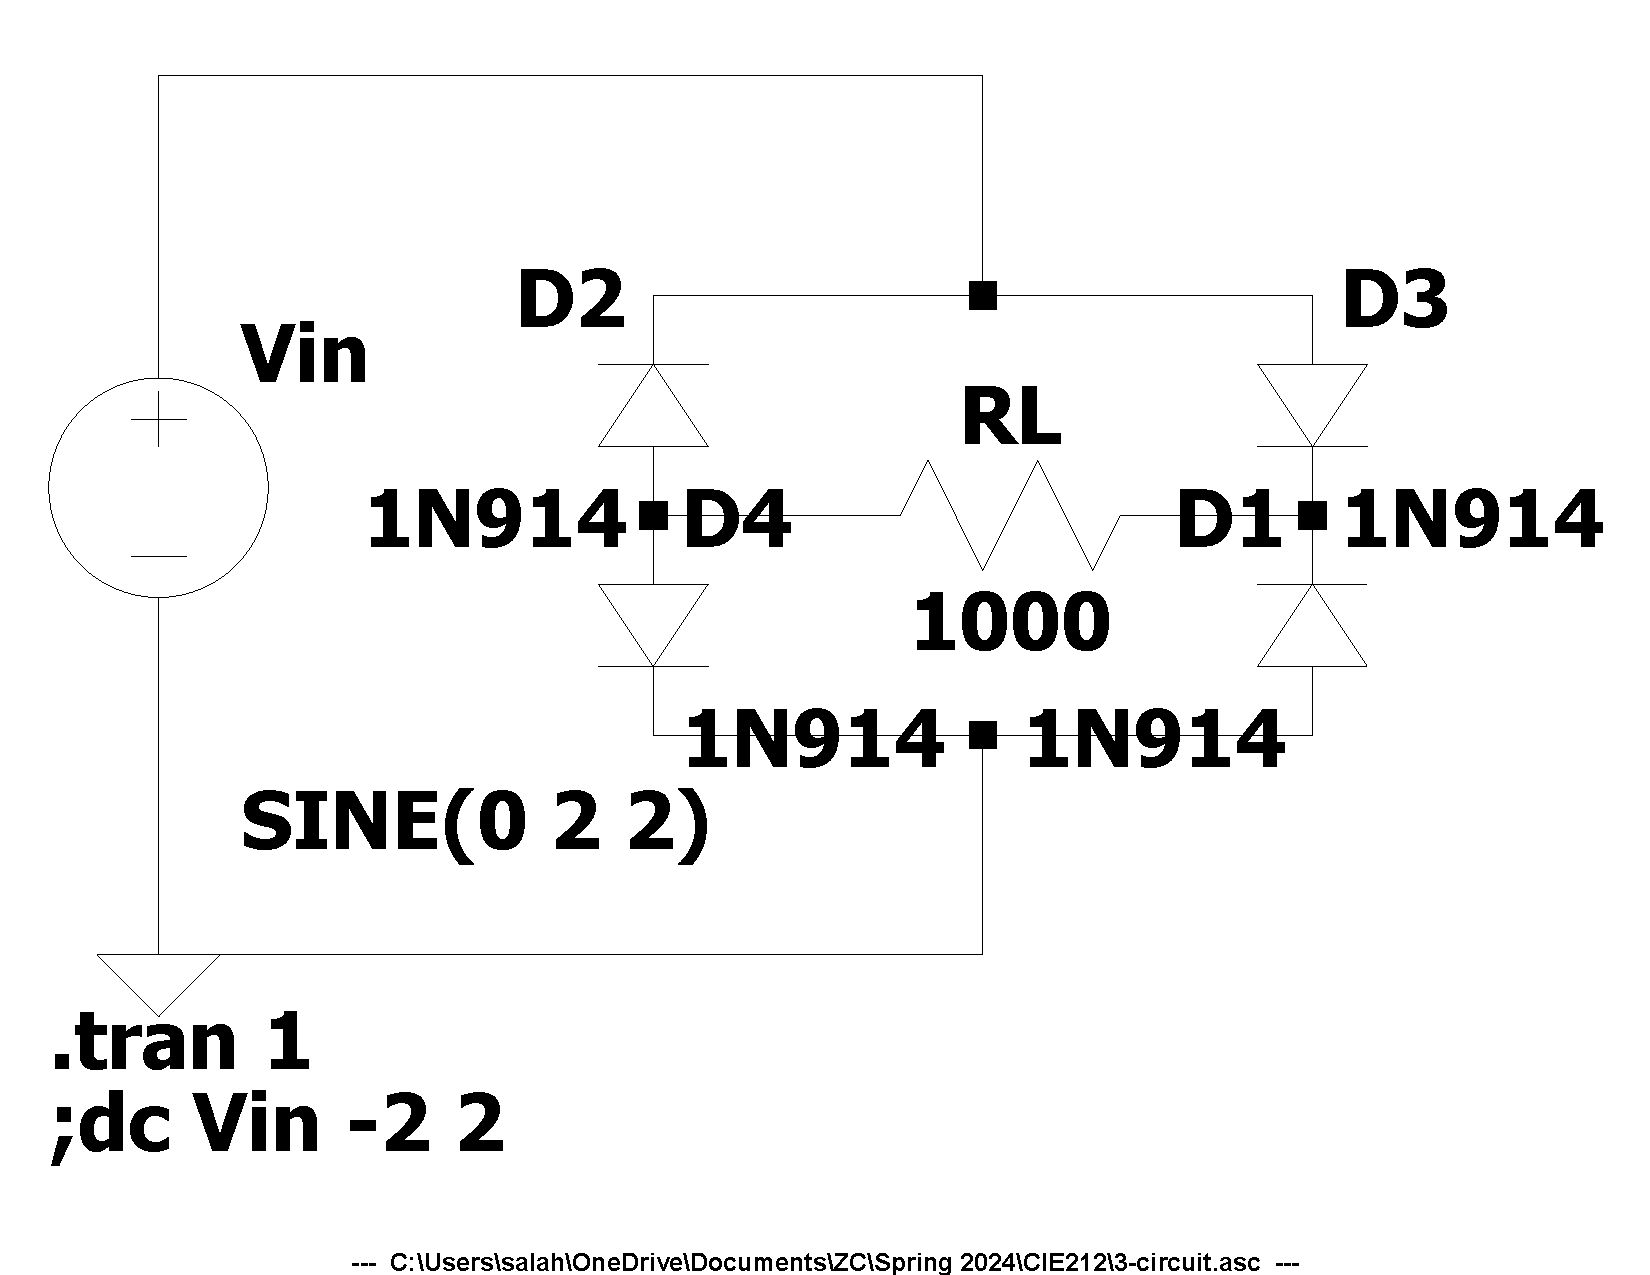
\includegraphics[width=0.95\textwidth]{figures/3-circuit.pdf}
      \caption{Circuit Diagram}
    \end{figure}
    \begin{figure}[H]
      \centering
      \begin{subfigure}{0.45\textwidth}
        \centering
        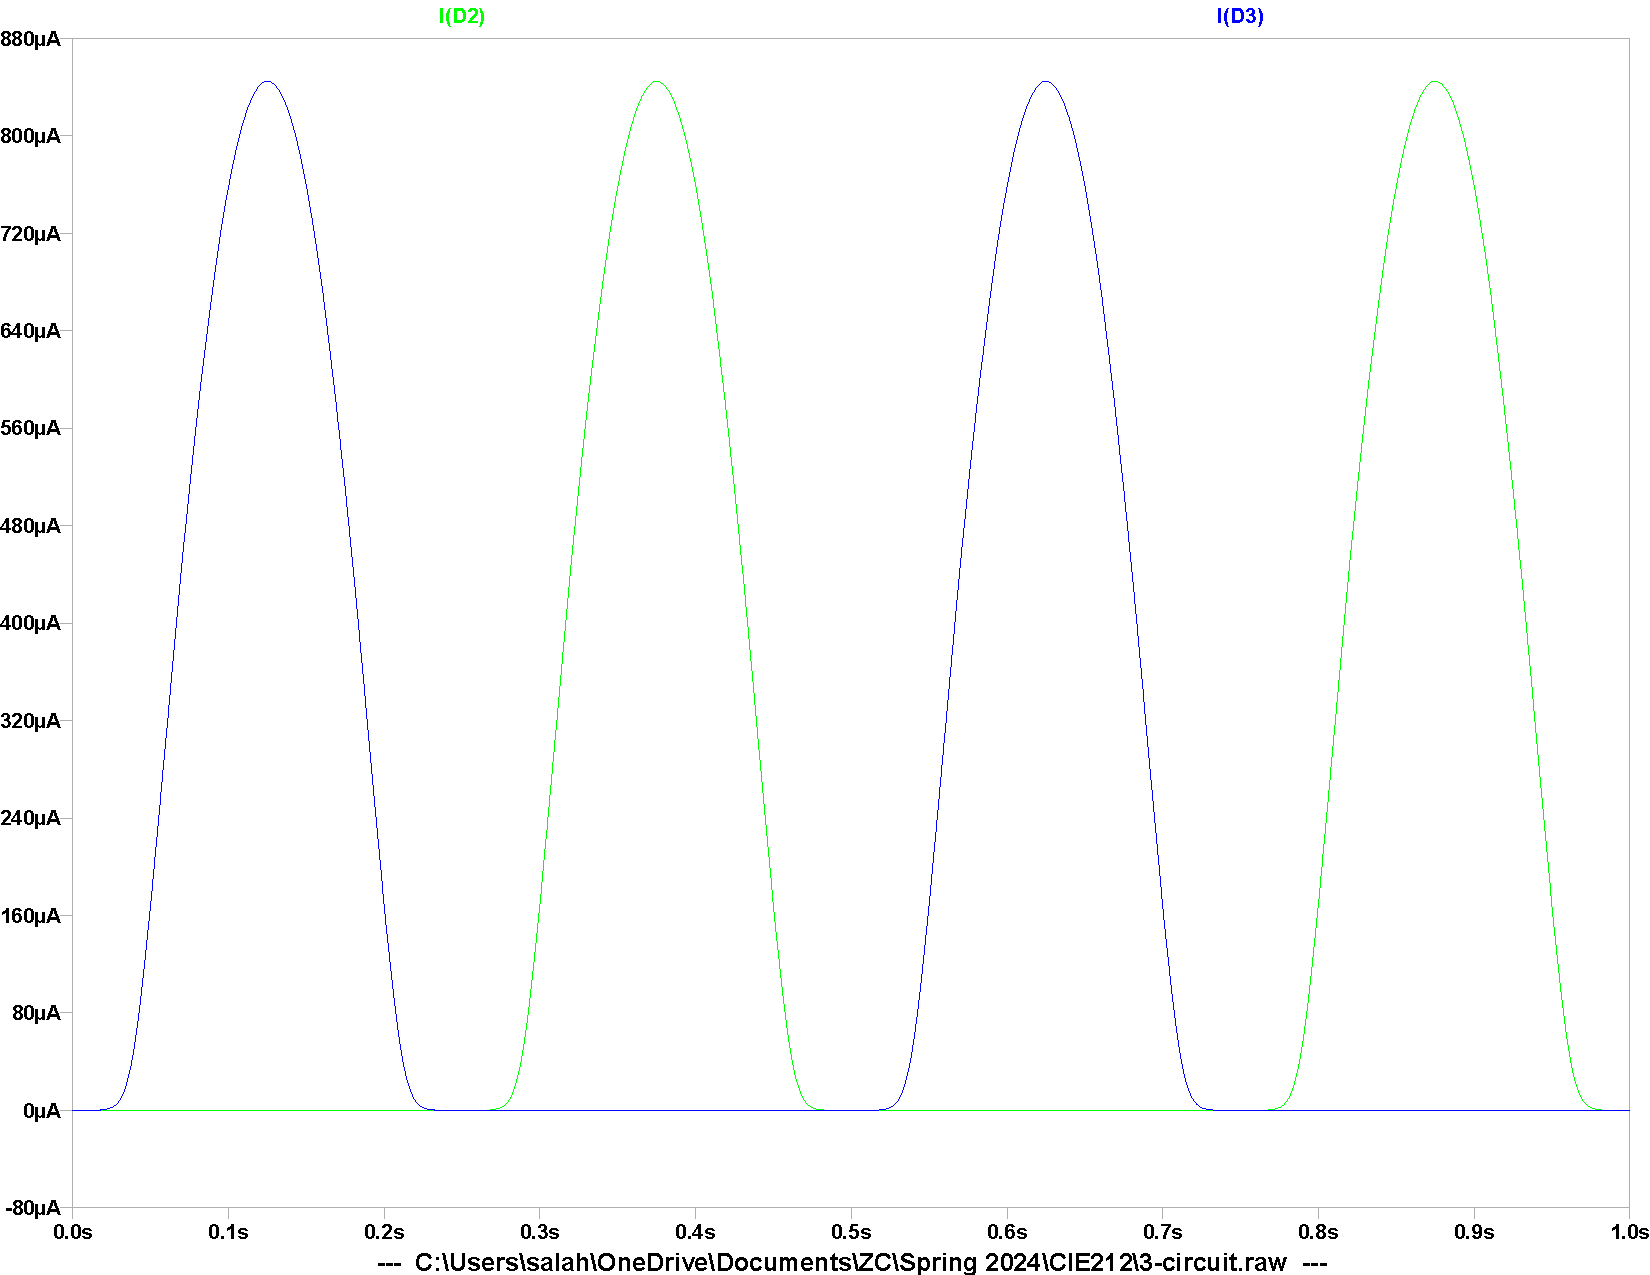
\includegraphics[width=\textwidth]{figures/3-transient-1.pdf}
        \caption{Transient Analysis 1}
      \end{subfigure}%
      \vspace{1cm}
      \begin{subfigure}{0.45\textwidth}
        \centering
        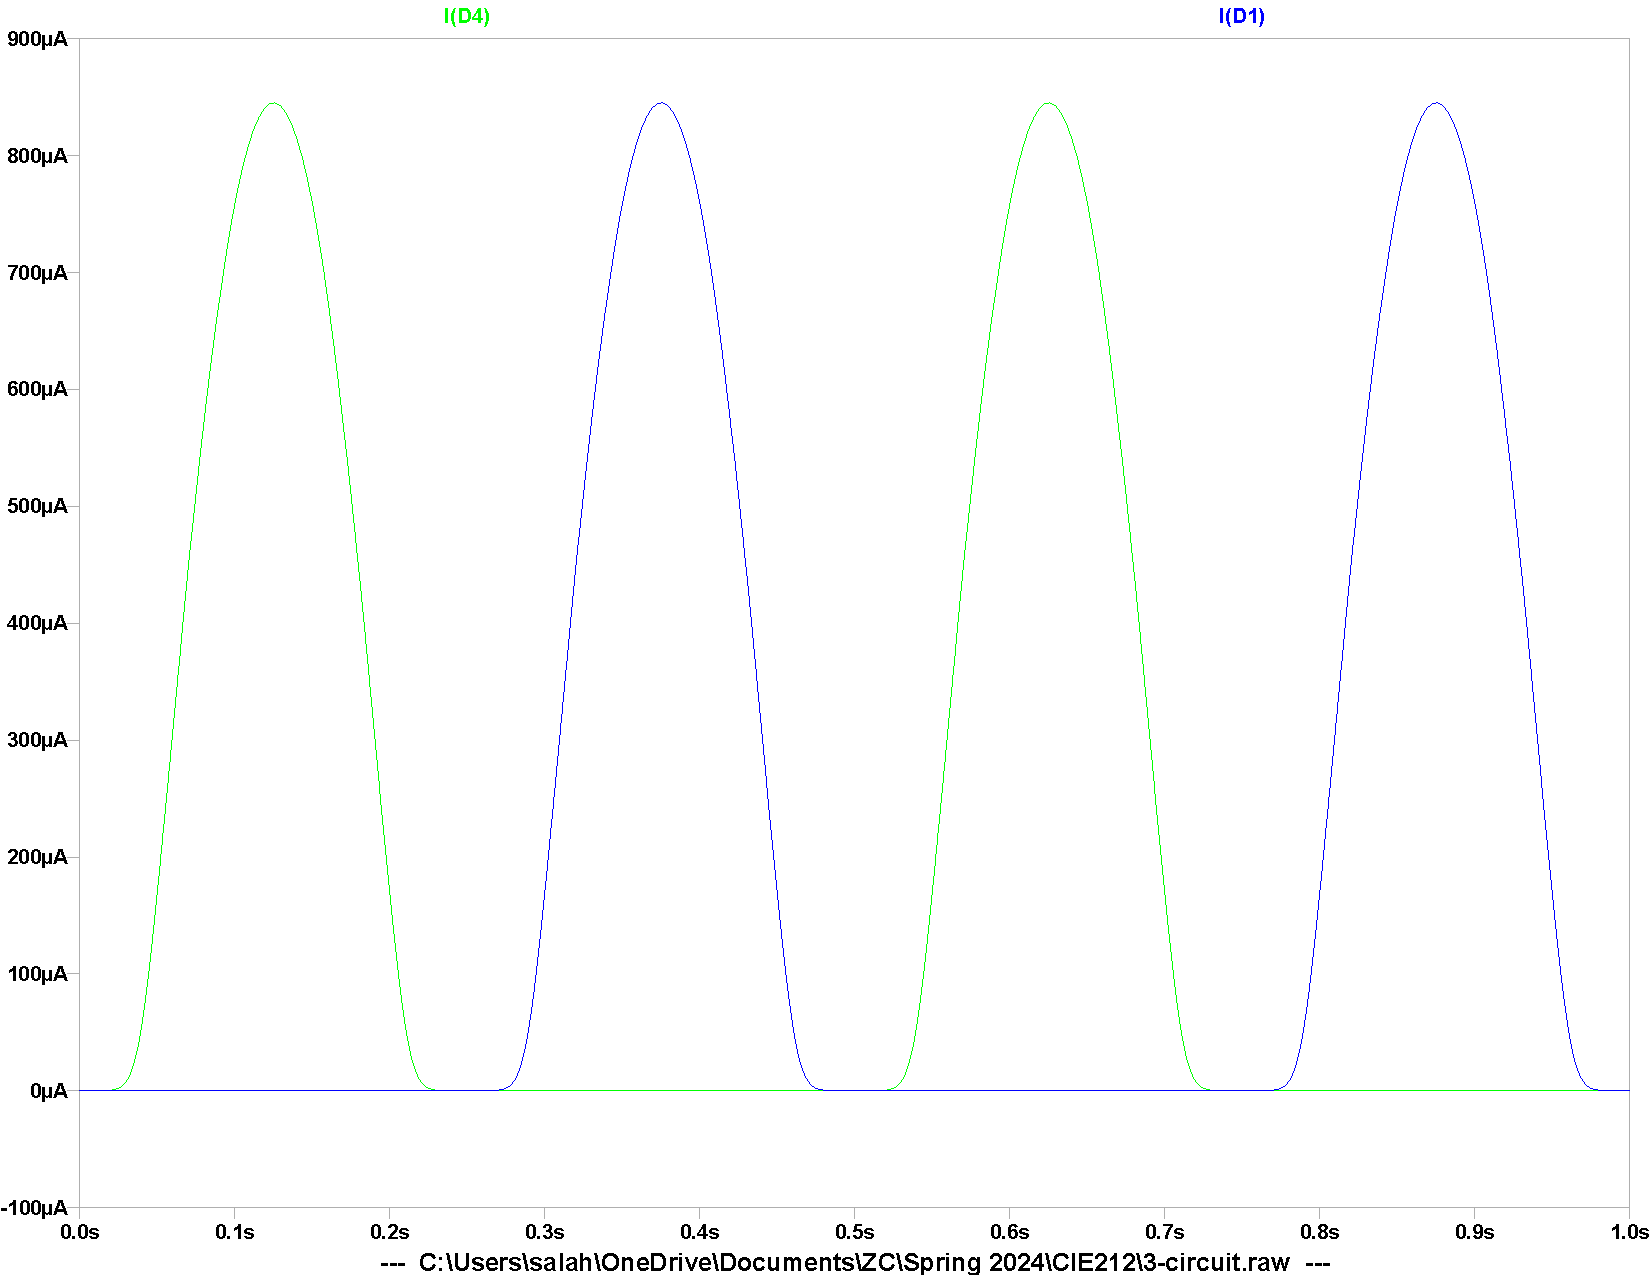
\includegraphics[width=\textwidth]{figures/3-transient-2.pdf}
        \caption{Transient Analysis 2}
      \end{subfigure}
      \caption{Simulation Results}
    \end{figure}

\end{enumerate}

\end{document}
